\documentclass[../differential_methods.tex]{subfiles}
\begin{document}
\section{Aula 03 - 09 de Março, 2026}
\subsection{Motivações}
\begin{itemize}
	\item Sistemas Expandidos;
	\item Condições de Fronteira Mistas;
	\item Problemas Bem-Postos.
\end{itemize}
\subsection{Sistemas Expandidos}
Em algumas situações, o uso de sistemas aumentados ou expandidos pode tornar a implementação como programa mais fácil ao incorporar equações para as condições de fronteira de sistemas lineares \(AU = F\) e incluir as variáveis desconhecidas das condições de fronteiras juntas! (``Adicionar os pontos \(0\) e \(m+1\)''); por exemplo, para os problemas de fronteira do tipo de Dirichlet, teríamos \(U_{0}=\alpha \) e \(U_{m+1}=\beta \), resultando no sistema linear expandido torna-se
\[
	A = \frac{1}{h^{2}}\begin{bmatrix}
		h^{2}  & 0      & \dotsc &        &        &       \\
		1      & -2     & 1      & \dotsc &        &       \\
		       & 1      & -2     & 1      & \dotsc &       \\
		\vdots & \vdots & \ddots & \ddots & \ddots &       \\
		       &        &        & 1      & -2     & 1     \\
		       &        &        &        & 0      & h^{2}
	\end{bmatrix}, \; U = \begin{bmatrix}
		U_{0}  \\
		U_{1}  \\
		U_{2}  \\
		\vdots \\
		U_{m}  \\
		U_{m+1}
	\end{bmatrix},\; F = \begin{bmatrix}
		\alpha   \\
		f(x_1)   \\
		f(x_2)   \\
		\vdots   \\
		f(x_{m}) \\
		\beta
	\end{bmatrix}.
\]
No entanto, não são todos os casos em que vamos ter condições de Fronteira de Dirichlet, e isso requer modificações do sistema expandido.

\begin{tcolorbox}[
		skin=enhanced,
		title=Lembrete!,
		after title={\hfill Condições de Contorno},
		fonttitle=\bfseries,
		sharp corners=downhill,
		colframe=black,
		colbacktitle=yellow!75!white,
		colback=yellow!30,
		colbacklower=black,
		coltitle=black,
		%drop fuzzy shadow,
		drop large lifted shadow
	]
	Alguns exemplos de condições de contorno que garantem o requerimento acima são:
	\begin{align*}
		 & u(0) = u(L) = v(0) = v(L) = 0 \text{ (Dirichlet)}                                  \\
		 & u'(0) = u'(L) = v'(0) = v'(L) = 0 \text{ (Neumann)}                                \\
		 & u(0) = u(L),\; u'(0) = u'(L), \; v(0) = v(L),\; v'(0) = v'(L) \text{ (Periódica)}.
	\end{align*}

	Em geral, definimos as \hypertarget{boundary_conditions}{condições de contorno} da seguinte forma:
	\[
		\mathcal{C}u = 0 \Longleftrightarrow \left\{\begin{array}{ll}
			\alpha_1 u(0) + \tilde{\alpha }_1u'(0) + \beta_1u(L) + \tilde{\beta }_1u'(L) = 0 \\
			\alpha_2 v(0) + \tilde{\alpha }_2v'(0) + \beta_2v(L) + \tilde{\beta }_2v'(L) = 0 \\
		\end{array}\right.,
	\]
	em que os coeficientes são reais e seus conjuntos como vetores, isto é,
	\[
		(\alpha_1, \tilde{\alpha }_1, \beta_1, \tilde{\beta }_1) \quad\&\quad (\alpha_2, \tilde{\alpha }_2, \beta_2, \tilde{\beta }_2)
	\]
	são linearmente independentes. Queremos que, se u e v forem funções de classe \(\mathcal{C}^{2}([0, L])\) satisfazem \(\mathcal{C}u_1 = \mathcal{C}u_2 = 0\), então
	\[
		u'(L)v(L) - u'(0)v'(0) - u(L)v'(L) + u(0)v'(0) = 0.
	\]
\end{tcolorbox}

Vamos considerar a equação diferencial de segunda ordem dada por
\[
	u''(x) = f(x), \quad 0<x<1,
\]
com condição de fronteira de Neumann na fronteira com 0, \(u'(0)= \sigma \), e de Dirichlet na fronteira direita, \(u(1)=\beta \). Nesta situação, \(u(0)\) tornou-se uma incógnita, e a aproximação \(U_{0}\), consequentemente, também! Temos que dar um jeito de aproximar a condição \(u'(0)=\sigma \) e de modificarmos, de acordo com ela, a primeira linha do sistema expandido.

Utilizando a aproximação da derivada unilateral
\[
	u'(0)\approx D_{+}u(x_{0}) = \frac{u(x_1)-u(x_{0})}{h},
\]
obtemos a relação
\[
	\frac{U_1-U_0}{h} = \sigma ,
\]
mas que tem uma aproximação apenas de ordem 1, já que, pelo erro de truncamento local,
\begin{align*}
	\tau_{0} = \frac{1}{h}(u(x_1)-u(x_{0}))-\sigma & = \frac{1}{h}\biggl(u(x_{0})+hu'(x_{0})+\frac{1}{2}h^{2}u''(x_{0}) + \mathcal{O}(h^{3})-u(x_{0})\biggr)-\sigma \\
	                                               & = u'(x_{0})+\frac{1}{2}hu''(x_{0})+\mathcal{O}(h^{2})-\sigma                                                   \\
	                                               & = \frac{1}{2}hu''(x_{0}) + \mathcal{O}(h^{2})                                                                  \\
	                                               & = \mathcal{O}(h).
\end{align*}
Com essa aproximação, ganhamos o sistema linear nas incógnitas \(U_{0}, \dotsc , U_{m+1}\) com um erro global de ordem um e devido a \(\tau_{0}=\mathcal{O}(h)\):
\[
	A = \frac{1}{h^{2}}\begin{bmatrix}
		-h     & h      & \dotsc &        &        &       \\
		1      & -2     & 1      & \dotsc &        &       \\
		       & 1      & -2     & 1      & \dotsc &       \\
		\vdots & \vdots & \ddots & \ddots & \ddots &       \\
		       &        &        & 1      & -2     & 1     \\
		       &        &        &        & 0      & h^{2}
	\end{bmatrix} \begin{bmatrix}
		U_{0}  \\
		U_{1}  \\
		U_{2}  \\
		\vdots \\
		U_{m}  \\
		U_{m+1}
	\end{bmatrix} = \begin{bmatrix}
		\sigma   \\
		f(x_1)   \\
		f(x_2)   \\
		\vdots   \\
		f(x_{m}) \\
		\beta
	\end{bmatrix}.
\]

De maneira parecida, mas usmando uma precisão de segunda ordem, podemos aproximar \(u'(0)=\sigma \) de forma centralizada ao introduzir mais uma incógnita, \(U_{-1}\), junto à relação
\begin{align*}
	 & \frac{1}{h^{2}}(U_{-1}-2U_{0}+U_1)=f(x_{0}),
	 & \frac{1}{2h}(U_{1}-U_{-1})=\sigma ,
\end{align*}
resultando em um sistema linear de m+3 equações com m+3 incógnitas. Por um processo de eliminação de incógnitas, remove-se \(U_{-1}\) acima e obtém-se a relação
\[
	\frac{1}{h}(-U_{0}+U_{1})=\sigma +\frac{h}{2}f(x_{0}),
\]
reduzindo o caso de m+3 equações com m+3 incógnitas para o original com m+2 de cada, escrito como
\[
	A = \frac{1}{h^{2}}\begin{bmatrix}
		-h     & h      & \dotsc &        &        &       \\
		1      & -2     & 1      & \dotsc &        &       \\
		       & 1      & -2     & 1      & \dotsc &       \\
		\vdots & \vdots & \ddots & \ddots & \ddots &       \\
		       &        &        & 1      & -2     & 1     \\
		       &        &        &        & 0      & h^{2}
	\end{bmatrix} \begin{bmatrix}
		U_{0}  \\
		U_{1}  \\
		U_{2}  \\
		\vdots \\
		U_{m}  \\
		U_{m+1}
	\end{bmatrix} = \begin{bmatrix}
		\sigma + \frac{h}{2}f(x_{0}) \\
		f(x_1)                       \\
		f(x_2)                       \\
		\vdots                       \\
		f(x_{m})                     \\
		\beta
	\end{bmatrix}.
\]

\begin{figure}[H]
	\begin{center}
		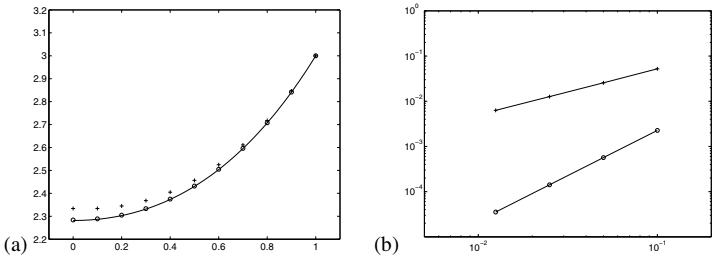
\includegraphics[height=\textheight, width=\textwidth, keepaspectratio]{./Images/ssheat_approxs_03.png}
	\end{center}
	\caption{A linha sólida é a solução real \(u(x)=e^{x}-x+4+e,\) o sinal + indica a solução numa malha de 20 pontos para a primeira abordagem, e o símbolo \(\circ \) é a segunda abordagem na mesma malha. Pelo gráfico log-log à direita, comparam-se os erros (na norma máxima).}
\end{figure}

\begin{tcolorbox}[
		skin=enhanced,
		title=Observação,
		fonttitle=\bfseries,
		colframe=black,
		colbacktitle=cyan!75!white,
		colback=cyan!15,
		colbacklower=black,
		coltitle=black,
		drop fuzzy shadow,
		%drop large lifted shadow
	]
	A matriz A é exatamente a mesma que a obtida na aproximação com precisão de primeira ordem, mas o lado direito da equação muda de \(\sigma \) para \(\sigma + \frac{h}{2}f(x_{0})\).

\end{tcolorbox}

Vale mencionar brevemente que teria como, ainda, fazer uma aproximação utilizando séries de Taylor:
\begin{align*}
	\frac{u(x_1)-u(x_{0})}{h}\approx u'\biggl(x_{0}+\frac{h}{2}\biggr) & = u'(x_{0})+\frac{h}{2}u''(x_{0}) + \mathcal{O}(h^{2}) \\
	                                                                   & = \sigma + \frac{h}{2}f(x_{0})+\mathcal{O}(h^{2}),
\end{align*}
ou até fazer uma aproximação de precisão de segunda ordem unilateral baseada nas três incógnitas \(U_0,\; U_1,\; U_2\):
\[
	\frac{1}{2h}(-3U_{0}+4U_{1}-U_{2})=\sigma \Longleftrightarrow  \frac{1}{h^{2}}\biggl(\frac{-3h}{2}U_{0}+2hU_{1}-\frac{h}{2}U_{2}\biggr) = \sigma.
\]
O problema é que o sistema linear resultante
\[
	A = \frac{1}{h^{2}}\begin{bmatrix}
		-\frac{3h}{2} & 2h     & -\frac{h}{2} & \dotsc &        &       \\
		1             & -2     & 1            & \dotsc &        &       \\
		              & 1      & -2           & 1      & \dotsc &       \\
		\vdots        & \vdots & \ddots       & \ddots & \ddots &       \\
		              &        &              & 1      & -2     & 1     \\
		              &        &              &        & 0      & h^{2}
	\end{bmatrix} \begin{bmatrix}
		U_{0}  \\
		U_{1}  \\
		U_{2}  \\
		\vdots \\
		U_{m}  \\
		U_{m+1}
	\end{bmatrix} = \begin{bmatrix}
		\sigma + \frac{h}{2}f(x_{0}) \\
		f(x_1)                       \\
		f(x_2)                       \\
		\vdots                       \\
		f(x_{m})                     \\
		\beta
	\end{bmatrix}
\]
sofre uma perturbação na sua estrutura tridiagonalizada, aumentando o custo computacional de resolver esse sistema.

\subsection{Problemas Bem-Postos}
Utilizando a definição de Jacques Hadamard,
\begin{def*}
	Uma modelagem matemática de um fenômeno físico é \textbf{bem-posta} (e deveria ser sempre que possível) se ela satisfaz:
	\begin{itemize}
		\item[1)] Uma solução existe;
		\item[2)] A solução é única; e
		\item[3)] O comportamento da solução muda de forma continua com os dados. \(\square\)
	\end{itemize}
\end{def*}
\begin{example}
	Até mesmo PVCs que parecem simples podem não ser bem-postos; basta considerar
	\[
		\left\{\begin{array}{ll}
			u''(x)=f(x),\quad 0<x<1 \\
			u'(0)=\sigma_{0}        \\
			u'(1)=\sigma_{1}
		\end{array}\right..
	\]
	Utilizando a abordagem de diferenças centradas para discretizar a equação diferencial e a segunda abordagem para lidar com os problemas de contorno do tipo Neumann, o sistema linear discreto resultante é da forma
	\[
		\frac{1}{h^{2}}\begin{bmatrix}
			-h     & h      & \dotsc &        &        &       \\
			1      & -2     & 1      & \dotsc &        &       \\
			       & 1      & -2     & 1      & \dotsc &       \\
			\vdots & \vdots & \ddots & \ddots & \ddots &       \\
			       &        &        & 1      & -2     & 1     \\
			       &        &        &        & 0      & h^{2}
		\end{bmatrix} \begin{bmatrix}
			U_{0}  \\
			U_{1}  \\
			U_{2}  \\
			\vdots \\
			U_{m}  \\
			U_{m+1}
		\end{bmatrix} = \begin{bmatrix}
			\sigma_{0} + \frac{h}{2}f(x_{0}) \\
			f(x_1)                           \\
			f(x_2)                           \\
			\vdots                           \\
			f(x_{m})                         \\
			-\sigma_{1}+\frac{h}{2}f(x_{m+1})
		\end{bmatrix},
	\]
	que é uma matriz singular e, em geral, ou ele não tem solução, ou ele tem infinitas soluções!

	A falha obtida na matriz do problema não é por conta do método numérico, mas sim porque ele em si não é bem-posto, e a equação diferencial definindo ele também terá nenhuma ou infinitas soluções! Tanto é que
	\[
		A[1,1,\dotsc ,1]^{T} = A \begin{bmatrix}
			1      \\
			1      \\
			\vdots \\
			1
		\end{bmatrix} = \begin{bmatrix}
			0      \\
			0      \\
			\vdots \\
			0
		\end{bmatrix}
	\]
\end{example}
A chave para a questão das soluções está em observar que alguns PVCs têm soluções únicas, enquanto que outros terão apenas se certas condições de solubilidade forem impostas, e isso dá dicas a um princípio geral importante conhecido como \textit{Alternativas de Fredholm}:
\hypertarget{fredholm_alternative}{
	\begin{theorem*}[Alternativas de Fredholm]
		Suponha que \(Ax = b\) é um sistema linear de m incógnitas e m equações. Então, vale exclusivamente uma das alternativas abaixo:
		\begin{itemize}
			\item[1)] Existe exatamente uma solução para cada b arbitrário (A é não-singular); Ou
			\item[2)] Existe uma solução não nula \(z\neq 0\) para \(Az=0\) (A é singular).
		\end{itemize}
	\end{theorem*}
}
Armados com essa ferramenta, vamos ver alguns casos de condições de fronteiras e equações diferenciais, junto à situação de suas soluções.

\textbf{\underline{Caso 1}:} o primeiro caso é uma barra isolada nas pontas, sem fluxo de calor nelas e sem fonte de calor por perto, ou seja,
\[
	\sigma_{0}=\sigma_{1}=0 \quad\&\quad f\equiv 0.
\]
Lembre-se que esse PVC é uma equação simplificada para encontrar as soluções de estado estacionário da equação
\[
	u_{t}(x, t)=\kappa u_{xx}(x, t)+\psi (x, t),\quad u(x,0)=u_{0}(x);
\]
sendo assim, como que \(u(x, t)\) muda com o passar do tempo?

Sabemos que a energia calórica total do sistema deve ser conservada ao longo do tempo, e que a difusão do calor tende a redistribuí-la até estar uniformemente distribuída pela barra, ou seja, esperamos uma solução de estado estacionário do tipo \(u(x)=c\). Logo, pela conservação de energia,
\[
	c = \int_{0}^{1}u_{0}(x) \mathrm{dx}.
\]
Porém, qualquer \(u(x)=c\) irá resolver esse sistema! Caímos no caso de infinitas soluções!

Nesse caso, o sistema físico tinha apenas uma solução, mas em nossa tentativa de simplificar ele resolvendo apenas na situação do estado estacionário, acabamos descartando uma informação essencial do sistema: quanto de calor estava disponível no início, ou seja, descartamos o dado inicial da equação de calor.

\textbf{\underline{Caso 2}:} a barra está com as pontas isoladas, sem fluxo de calor nelas, mas existe uma fonte de calor:
\[
	\sigma_{0}=\sigma_{1}=0 \quad\&\quad f\not\equiv 0.
\]
Se pedirmos que o calor esteja sendo constantemente adicionado à barra, ou seja, que \(f(x)<0\) em toda a parte. Já que nenhum calor está fugindo pelas pontas isoladas, o esperado é que a temperatura aumente indefinidamente -- nunca atingimos um estado estacionário, resultando numa falta de soluções para o PVC.

Por outro lado, se a fonte de calor for descrita por uma função positiva em parte do intervalo e negativa no restante, o efeito resultante da fonte fornecedora e do escape do fluxo de calor se cancelam! Daí, é possível que existe um estado estacionário. Nesse caso, integrando o PVC, observa-se que a solução existe somente se
\begin{align*}
	0=\sigma_{1}-\sigma_{0} & = u'(1)-u'(0)                    \\
	                        & = \int_{0}^{1}u''(x) \mathrm{dx} \\
	                        & = \int_{0}^{1}f(x) \mathrm{dx},
\end{align*}
ou seja, caímos novamente no caso de infinitas soluções. Na verdade, o estado inicial \(u(0)\) pode até mesmo ser arbitrário, pois:
\begin{align*}
	 & \int_{0}^{y}u''(s) \mathrm{d}s = \int_{0}^{y}f(s) \mathrm{d}s \Rightarrow u'(y)-u'(0)=\int_{0}^{y}f(s) \mathrm{d}s                                             \\
	 & \int_{0}^{x}u'(y) \mathrm{d}y=\int_{0}^{x}\int_{0}^{y}f(s) \mathrm{d}s \mathrm{d}y  \Rightarrow u(x)-u(0)=\int_{0}^{x}\int_{0}^{y}f(s) \mathrm{d}s \mathrm{d}y
\end{align*}
para qualquer \(u(0).\)

\textbf{\underline{Caso 3}:} as pontas \textbf{não} estão isoladas, ou seja, há fluxo de calor:
\[
	\sigma_{0}\neq 0 \text{ e/ ou } \sigma_{1}\neq 0.
\]
Aqui, por conta da existência do fluxo de calor na fronteira, o calor da fonte deve cancelar o fluxo nas fronteiras; como
\[
	u'(1)-u'(0)=\int_{0}^{1}u''(x) \mathrm{d}x = \int_{0}^{1}f(x) \mathrm{d}x,
\]
devemos ter
\[
	\int_{0}^{1}f(x) \mathrm{d}x =\sigma_1-\sigma_{0},
\]
fornecendo infinitas soluções, porque, novamente, \(u(0)\) pode ser qualquer coisa:
\begin{align*}
	\int_{0}^{y}u''(s) \mathrm{d}s = \int_{0}^{y}f(s) \mathrm{d}s & \Rightarrow u'(y)-u'(0)=\int_{0}^{y}f(s) \mathrm{d}s                                                         \\
	                                                              & \Rightarrow u'(y)=\sigma_{0}+\int_{0}^{y}f(s) \mathrm{d}s                                                    \\
	                                                              & \Rightarrow \int_{0}^{x}u'(y) \mathrm{d}y = \sigma_{0}x+\int_{0}^{x}\int_{0}^{y}f(s) \mathrm{d}s \mathrm{d}y \\
	                                                              & \Rightarrow u(x)=u(0)+\sigma_{0}x+\int_{0}^{x}\int_{0}^{y}f(s) \mathrm{d}s \mathrm{d}y.
\end{align*}

Similarmente aos casos, o sistema singular expandido
\[
	\frac{1}{h^{2}}\begin{bmatrix}
		-h     & h      & \dotsc &        &        &       \\
		1      & -2     & 1      & \dotsc &        &       \\
		       & 1      & -2     & 1      & \dotsc &       \\
		\vdots & \vdots & \ddots & \ddots & \ddots &       \\
		       &        &        & 1      & -2     & 1     \\
		       &        &        &        & 0      & h^{2}
	\end{bmatrix} \begin{bmatrix}
		U_{0}  \\
		U_{1}  \\
		U_{2}  \\
		\vdots \\
		U_{m}  \\
		U_{m+1}
	\end{bmatrix} = \begin{bmatrix}
		\sigma_{0} + \frac{h}{2}f(x_{0}) \\
		f(x_1)                           \\
		f(x_2)                           \\
		\vdots                           \\
		f(x_{m})                         \\
		-\sigma_{1}+\frac{h}{2}f(x_{m+1})
	\end{bmatrix}
\]
terá uma solução (na verdade, infinitas) somente se F é ortogonal ao espaço anulador de \(A^{T}\). Com efeito, supondo que temos uma solução \(U\) e que \(A^{T}V=0\), então
\[
	\langle F, V \rangle = \langle AU, V \rangle = \langle U, A^{T}V \rangle = \langle U, 0 \rangle = 0.
\]
\begin{tcolorbox}[
		skin=enhanced,
		title=Observação,
		fonttitle=\bfseries,
		colframe=black,
		colbacktitle=cyan!75!white,
		colback=cyan!15,
		colbacklower=black,
		coltitle=black,
		drop fuzzy shadow,
		%drop large lifted shadow
	]
	Observe aqui que temos
	\[
		A^{T}\begin{bmatrix}
			1      \\
			h      \\
			\vdots \\
			h      \\
			1
		\end{bmatrix}=0,
	\]
	fornecendo a condição
	\[
		\langle F, V \rangle=0 \Rightarrow \frac{h}{2}\biggl(f(x_{0})+2 \sum\limits_{i=1}^{m}f(x_{i}) + f(x_{m+1})\biggr) = \sigma_1-\sigma_{0},
	\]
	que é exatamente a regra do trapezoide para a aproximação de
	\[
		\int_{0}^{1}f(x) \mathrm{d}x = \sigma_{1}-\sigma_{0}.
	\]
\end{tcolorbox}

\end{document}
